\documentclass[a4paper,11pt]{article}
\usepackage{graphicx}
\usepackage{subcaption} %subsection
\usepackage[english]{babel} % mirror
% define the title
\author{A.~Faraz}
\title{Figures in \LaTeXe}

\begin{document}
\maketitle
\pagebreak
Figure \ref{fig:boat1} shows a boat.
	\begin{figure}[h!]
		\centering
		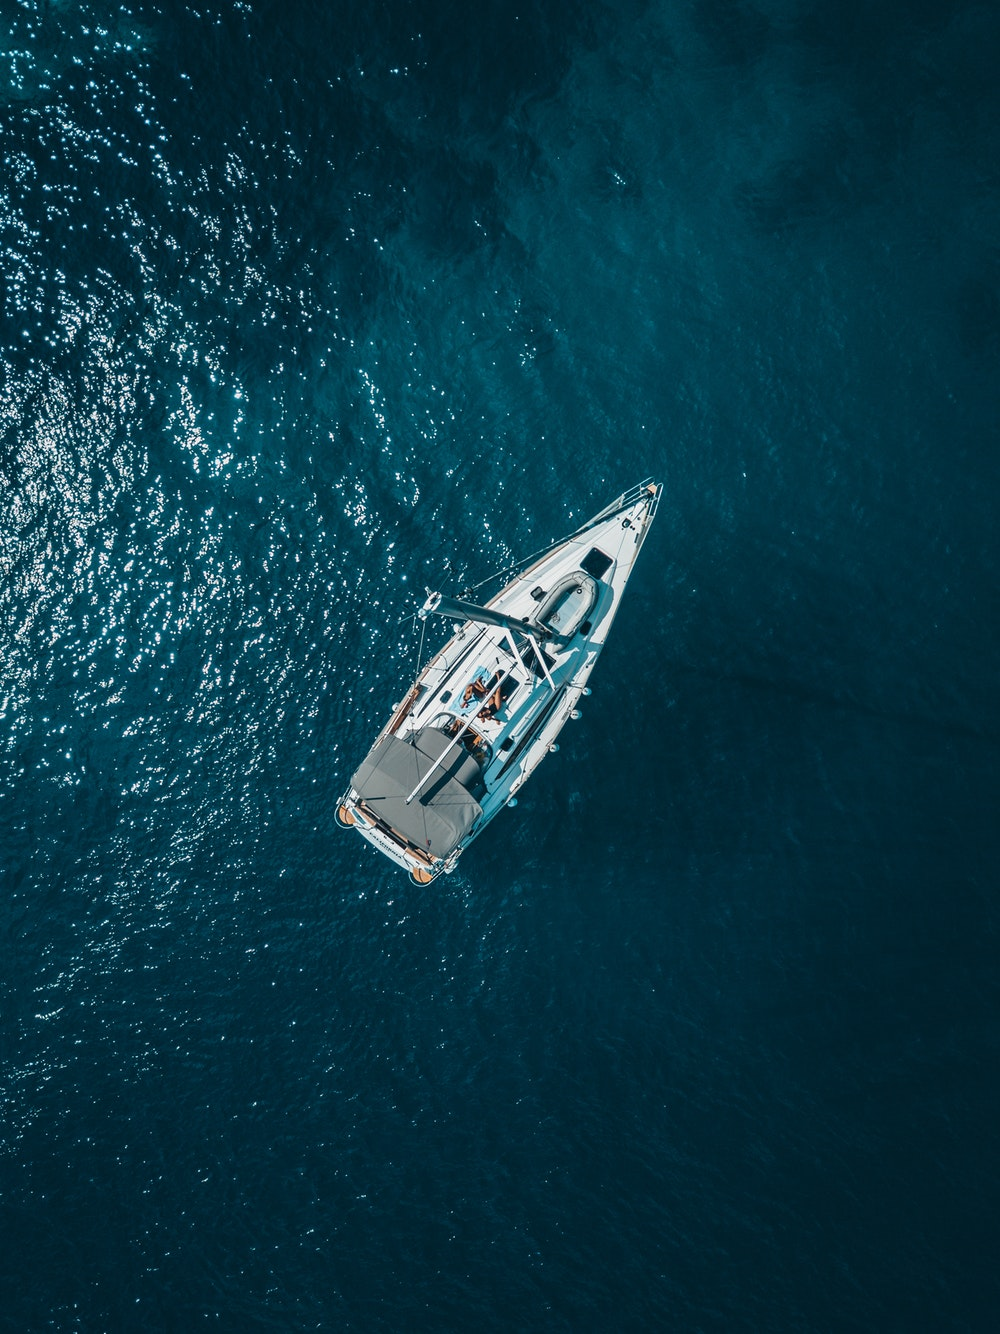
\includegraphics[width=0.5\linewidth]{boat.jpeg}
		\caption{A boat.}
		\label{fig:boat1}
	\end{figure}
% h -> here
% b -> buttom of page
% t -> top of page
% p -> on extra page
% ! -> override(will force specified location)
\pagebreak

\begin{figure}[h!]
	\centering
	\begin{subfigure}[b]{0.4\linewidth}
		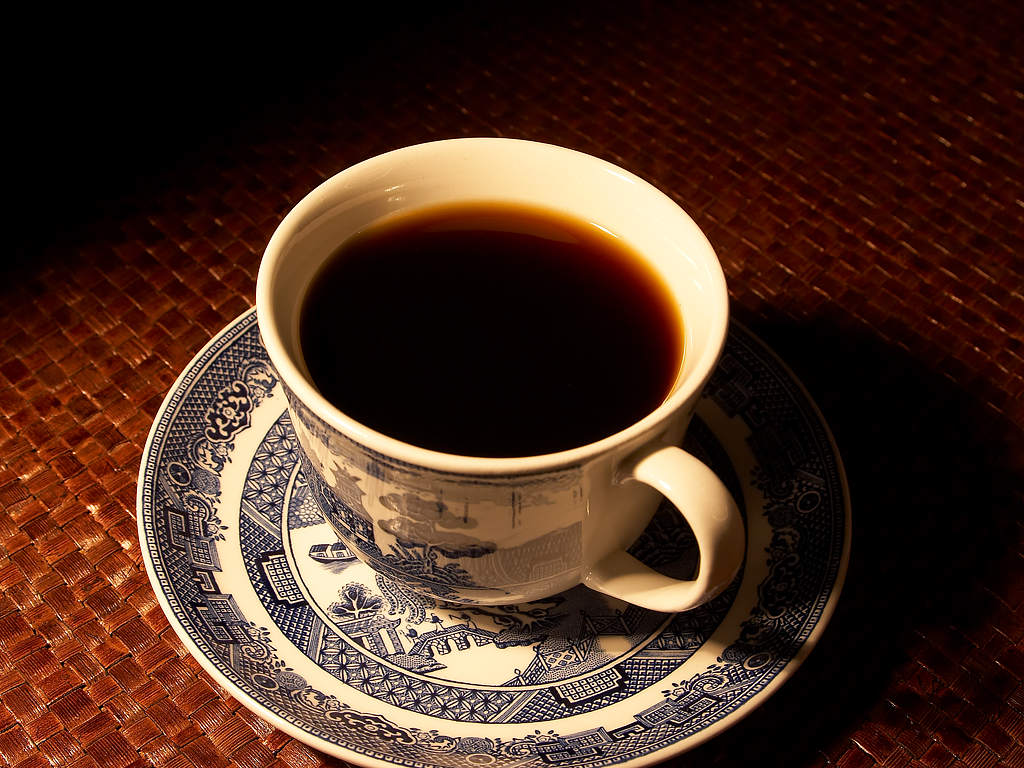
\includegraphics[width=\linewidth]{coffee.jpg}
		\caption{Coffee.}
	\end{subfigure}
	\begin{subfigure}[b]{0.4\linewidth}
		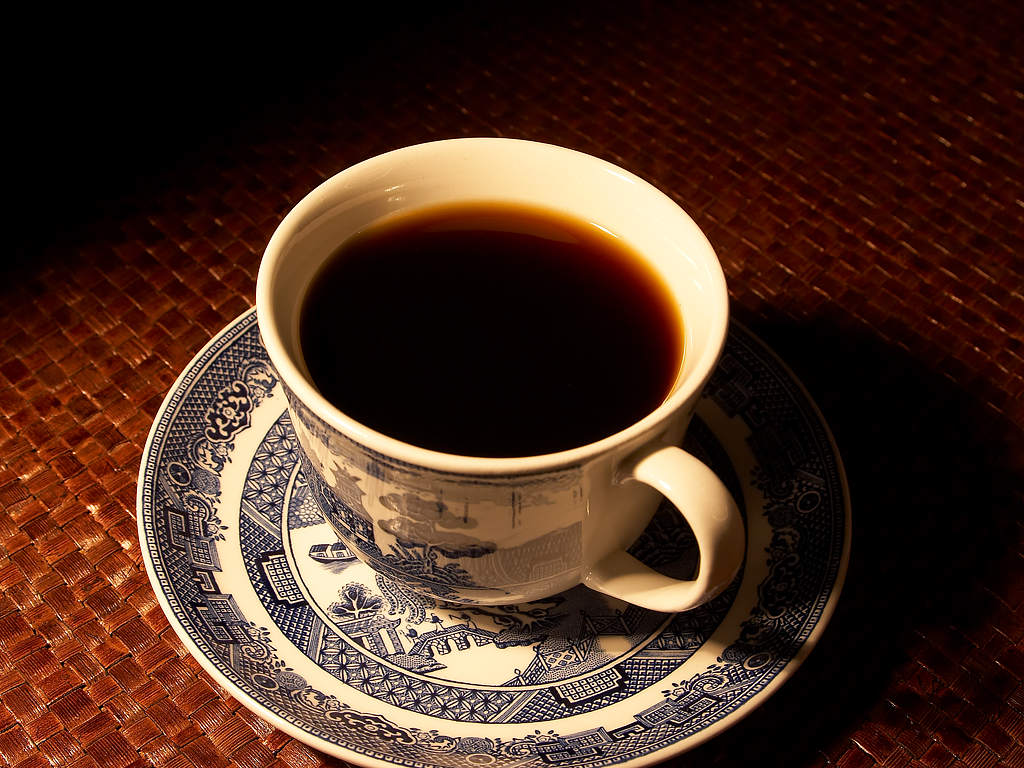
\includegraphics[width=\linewidth]{coffee.jpg}
		\caption{More coffee.}
	\end{subfigure}
	\caption{The same cup of coffee. Two times.}
	\label{fig:coffee}
\end{figure}

\pagebreak

\begin{figure}[h!]
	\centering
	\begin{subfigure}[b]{0.2\linewidth}
		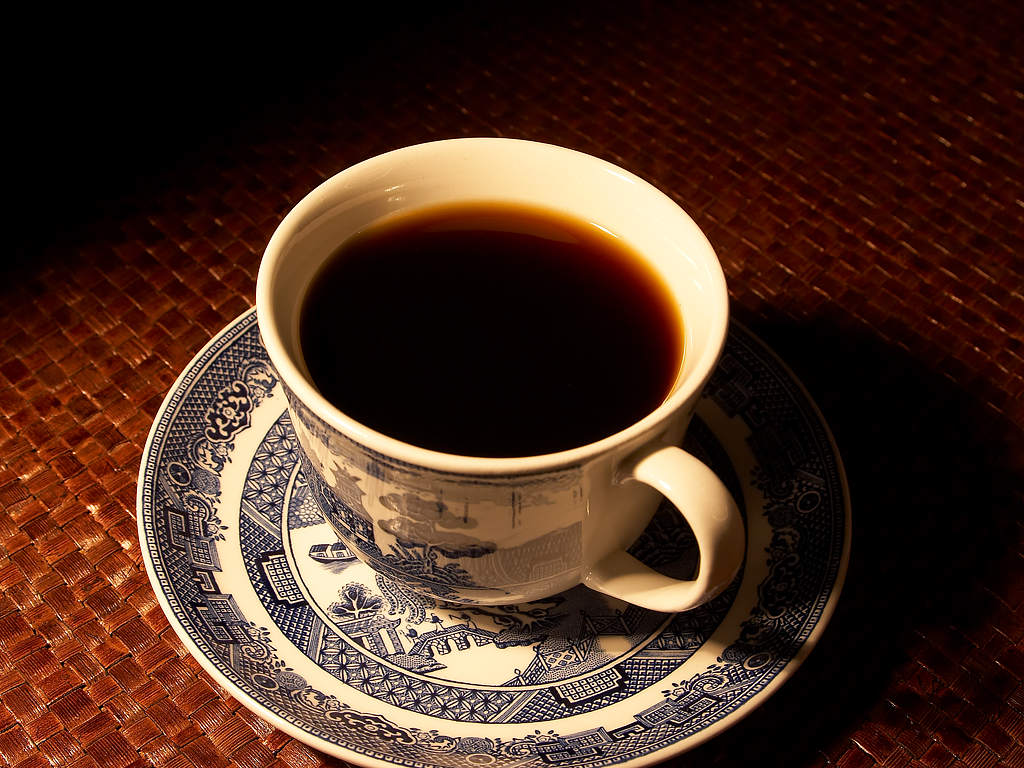
\includegraphics[width=\linewidth]{coffee.jpg}
		\caption{Coffee.}
	\end{subfigure}
	\begin{subfigure}[b]{0.2\linewidth}
		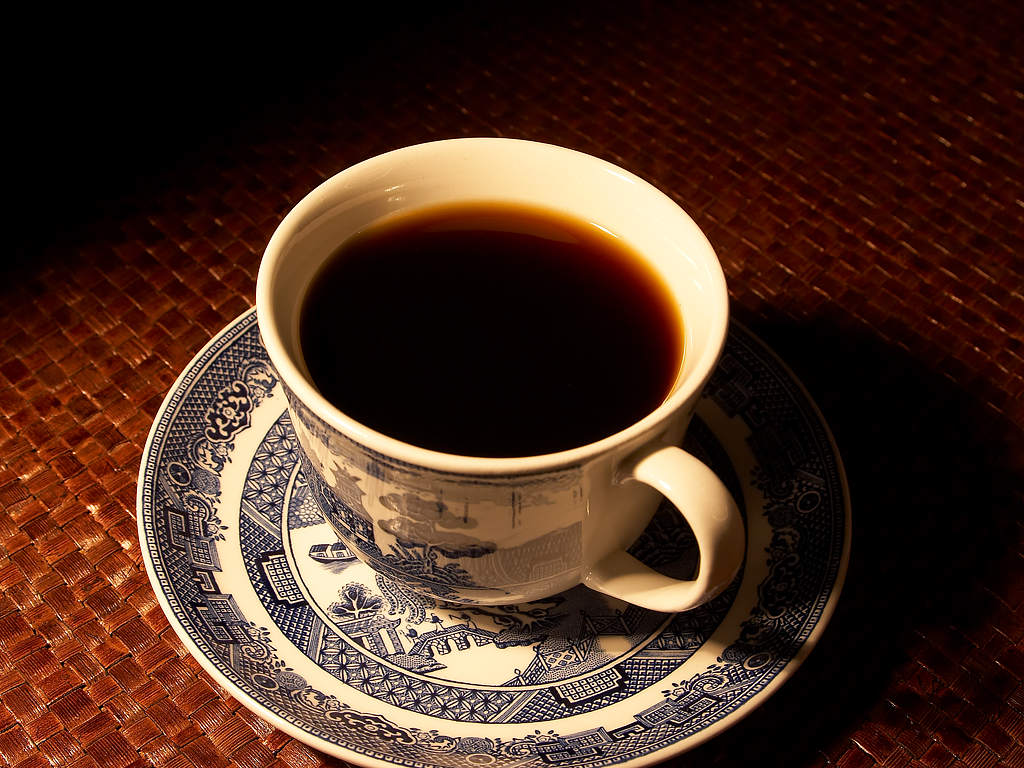
\includegraphics[width=\linewidth]{coffee.jpg}
		\caption{More coffee.}
	\end{subfigure}
	\begin{subfigure}[b]{0.2\linewidth}
		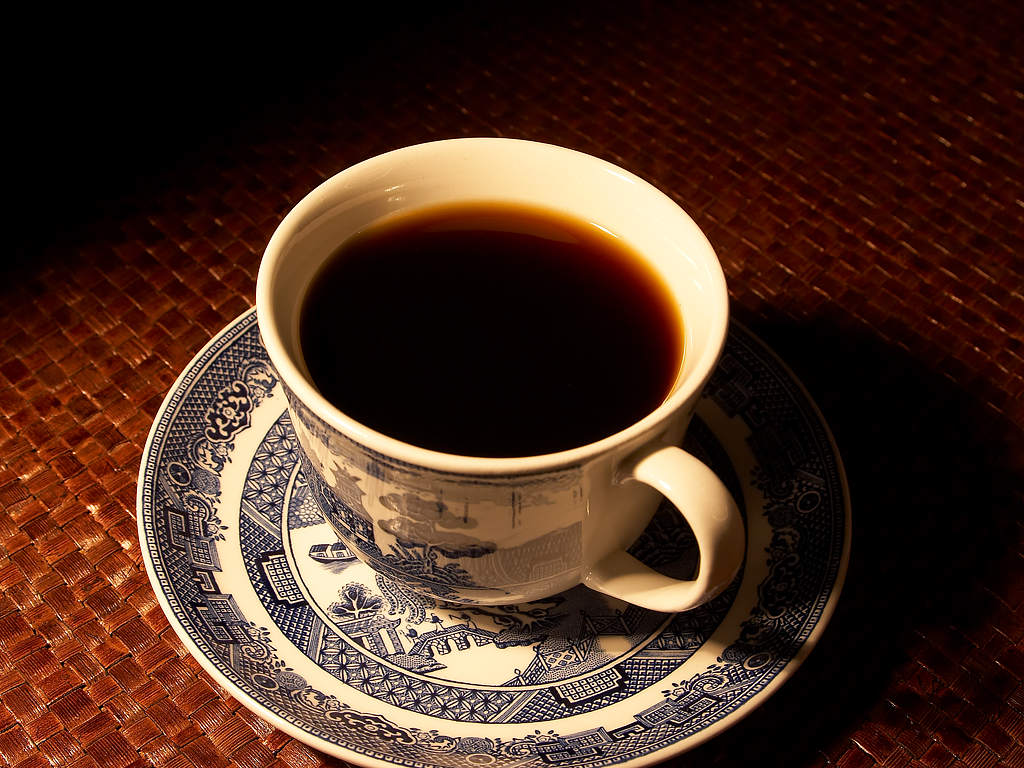
\includegraphics[width=\linewidth]{coffee.jpg}
		\caption{Tasty coffee.}
	\end{subfigure}
	
	\begin{subfigure}[b]{0.5\linewidth}
		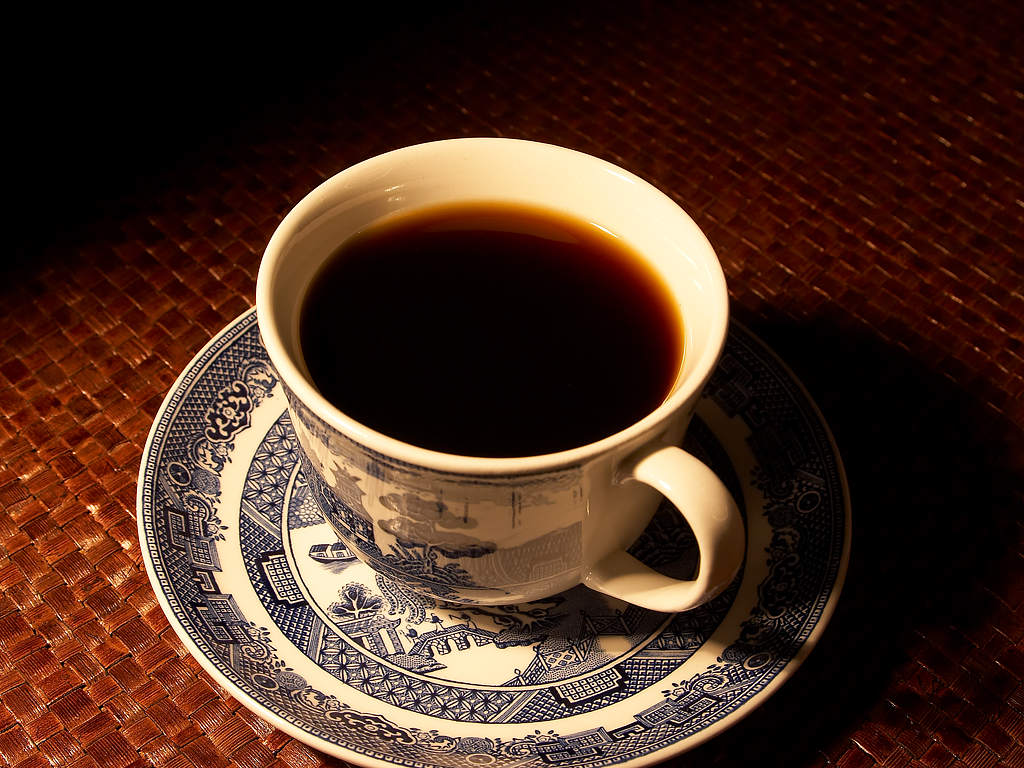
\includegraphics[width=\linewidth]{coffee.jpg}
		\caption{Too much coffee.}
	\end{subfigure}
	\caption{The same cup of coffee. Multiple times.}
	\label{fig:coffee3}
\end{figure}

\pagebreak


\begin{figure}
	\caption{A picture of an angry seagull.}
	\centering
	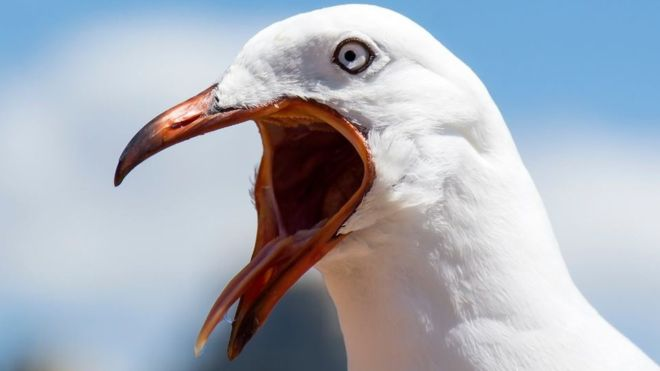
\includegraphics[width=0.5\textwidth]{angry.jpg}
\end{figure}
\begin{figure}
	\centering
	\reflectbox{%
		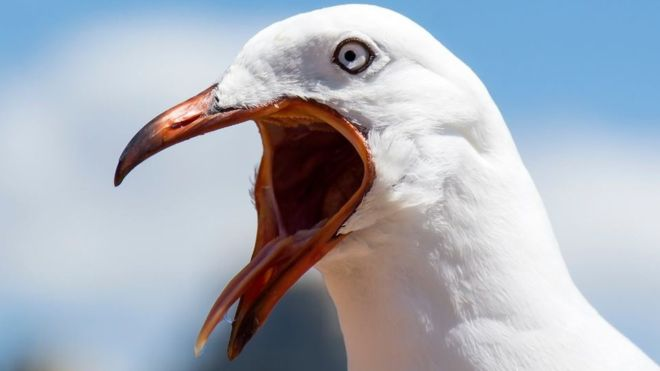
\includegraphics[width=0.5\textwidth]{angry.jpg}}
	\caption{A picture of the same seagull
		shouting the other way!}
\end{figure}

\pagebreak
\end{document}
